\begin{figure}
    \centering
    \begin{tabular}{c c c c}

        %  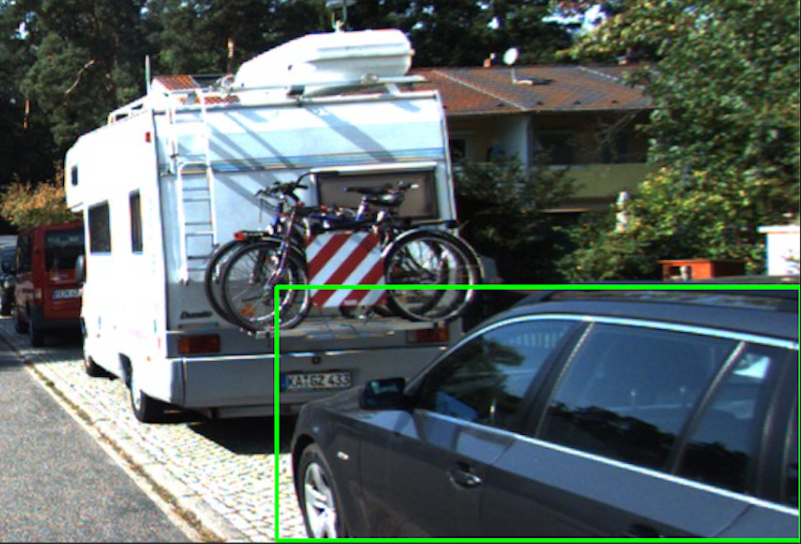
\includegraphics[width=0.2\textwidth]{figures/method/ambiguous/ex2/rgb.png}
        % &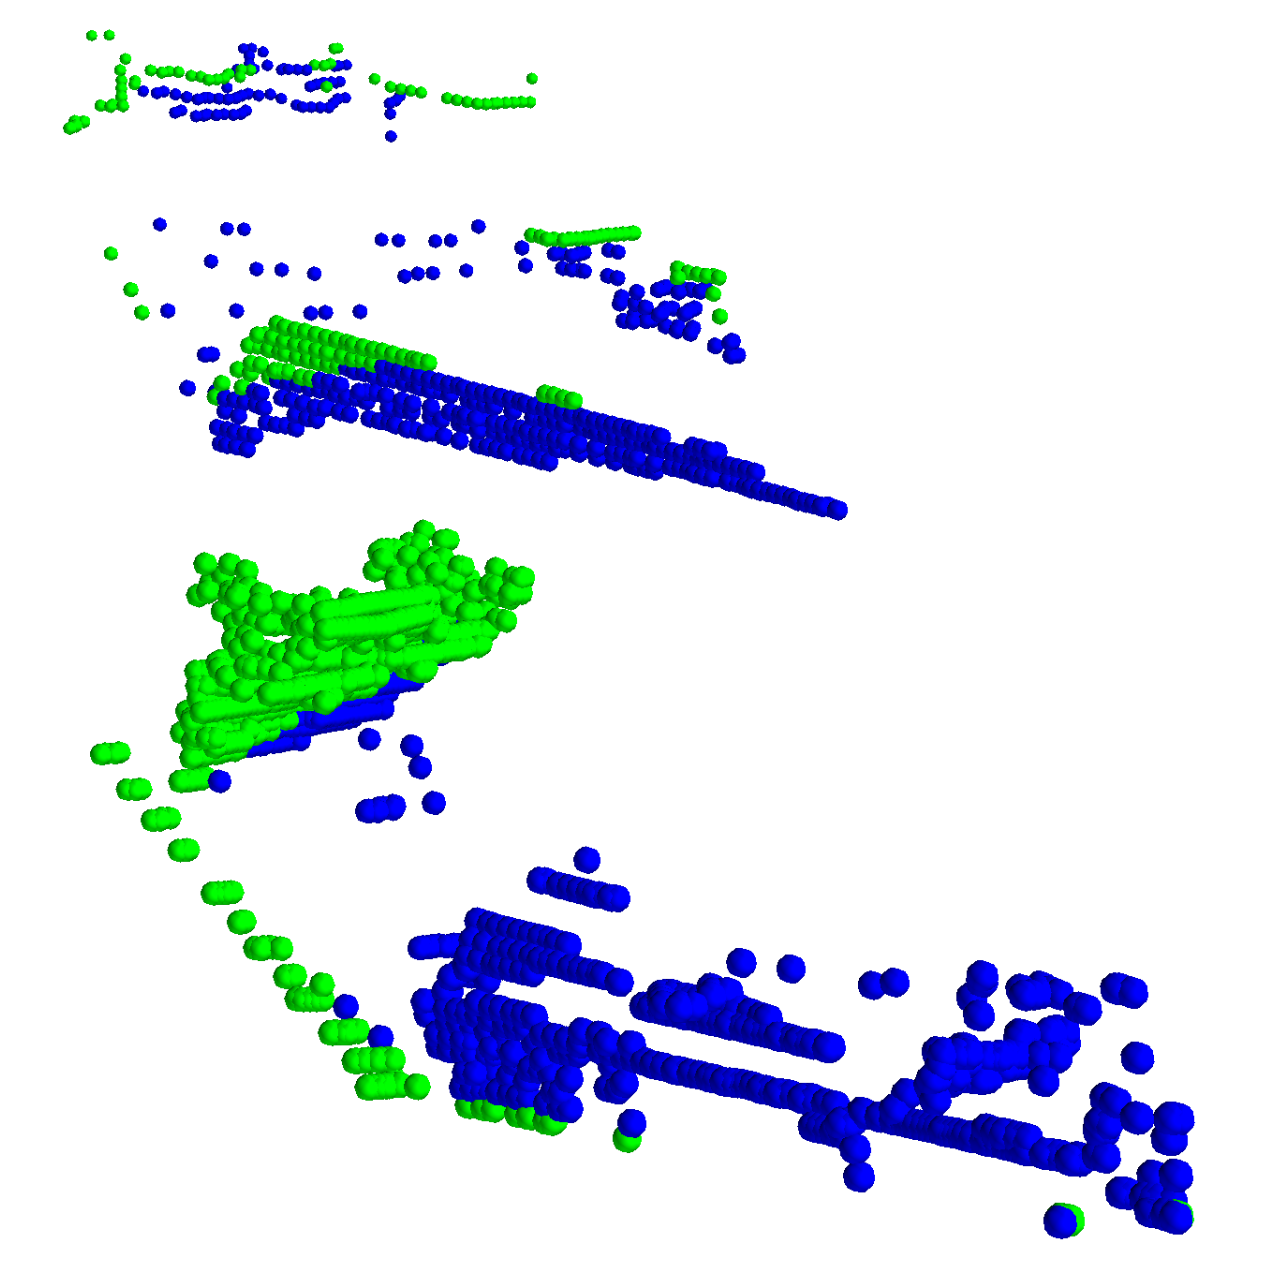
\includegraphics[width=0.2\textwidth]{figures/method/ambiguous/ex2/pcd.png} &
         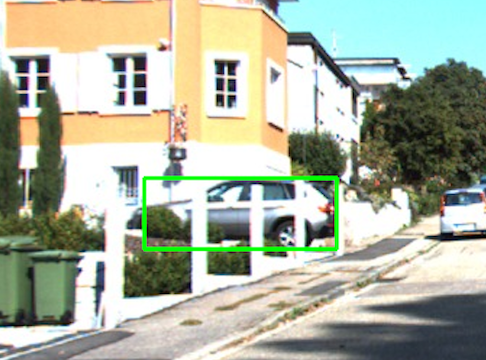
\includegraphics[width=0.2\textwidth]{figures/method/ambiguous/ex3/rgb.png}
        &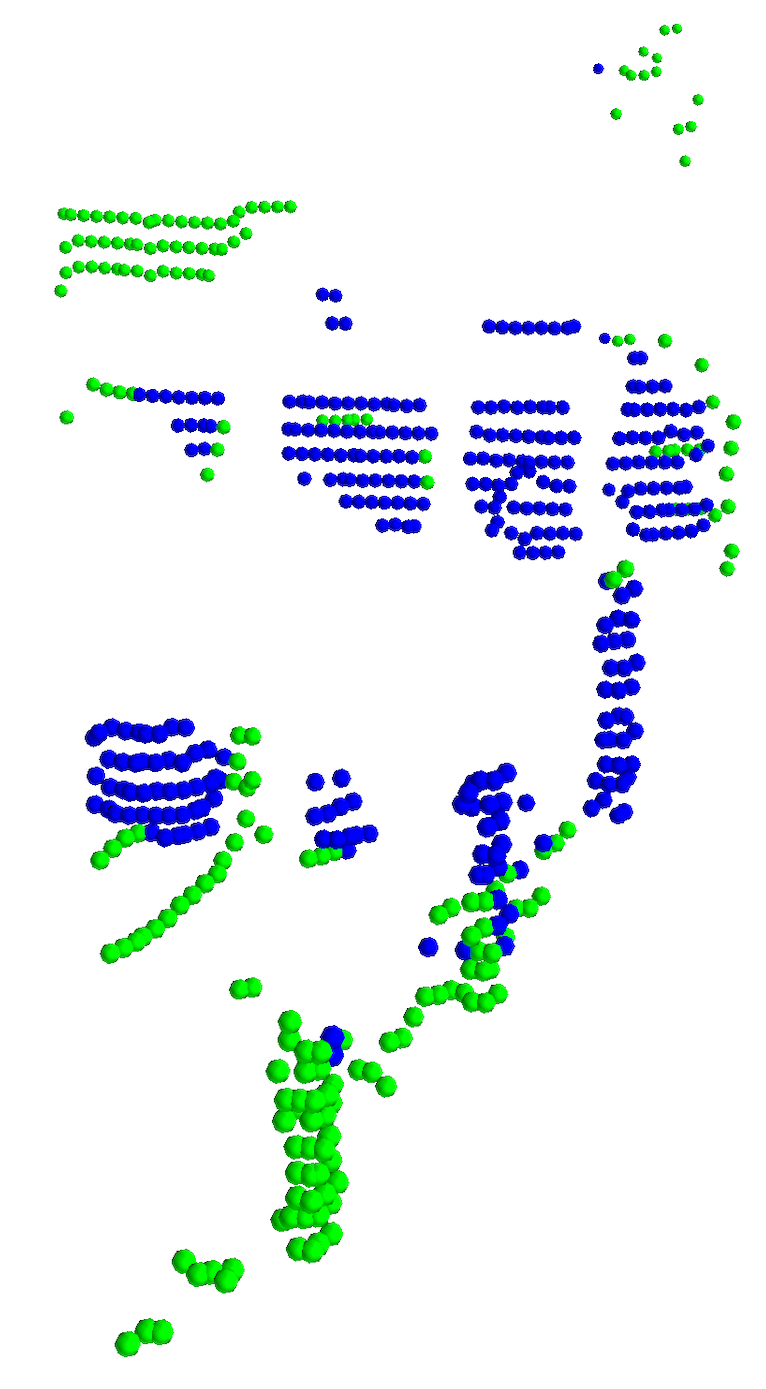
\includegraphics[width=0.1\textwidth]{figures/method/ambiguous/ex3/pcd.png} &
         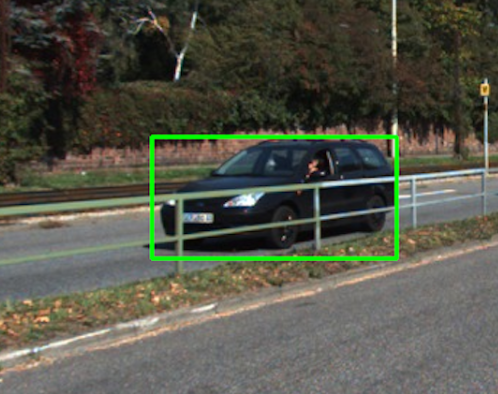
\includegraphics[width=0.2\textwidth]{figures/method/ambiguous/ex5/rgb.png}
        &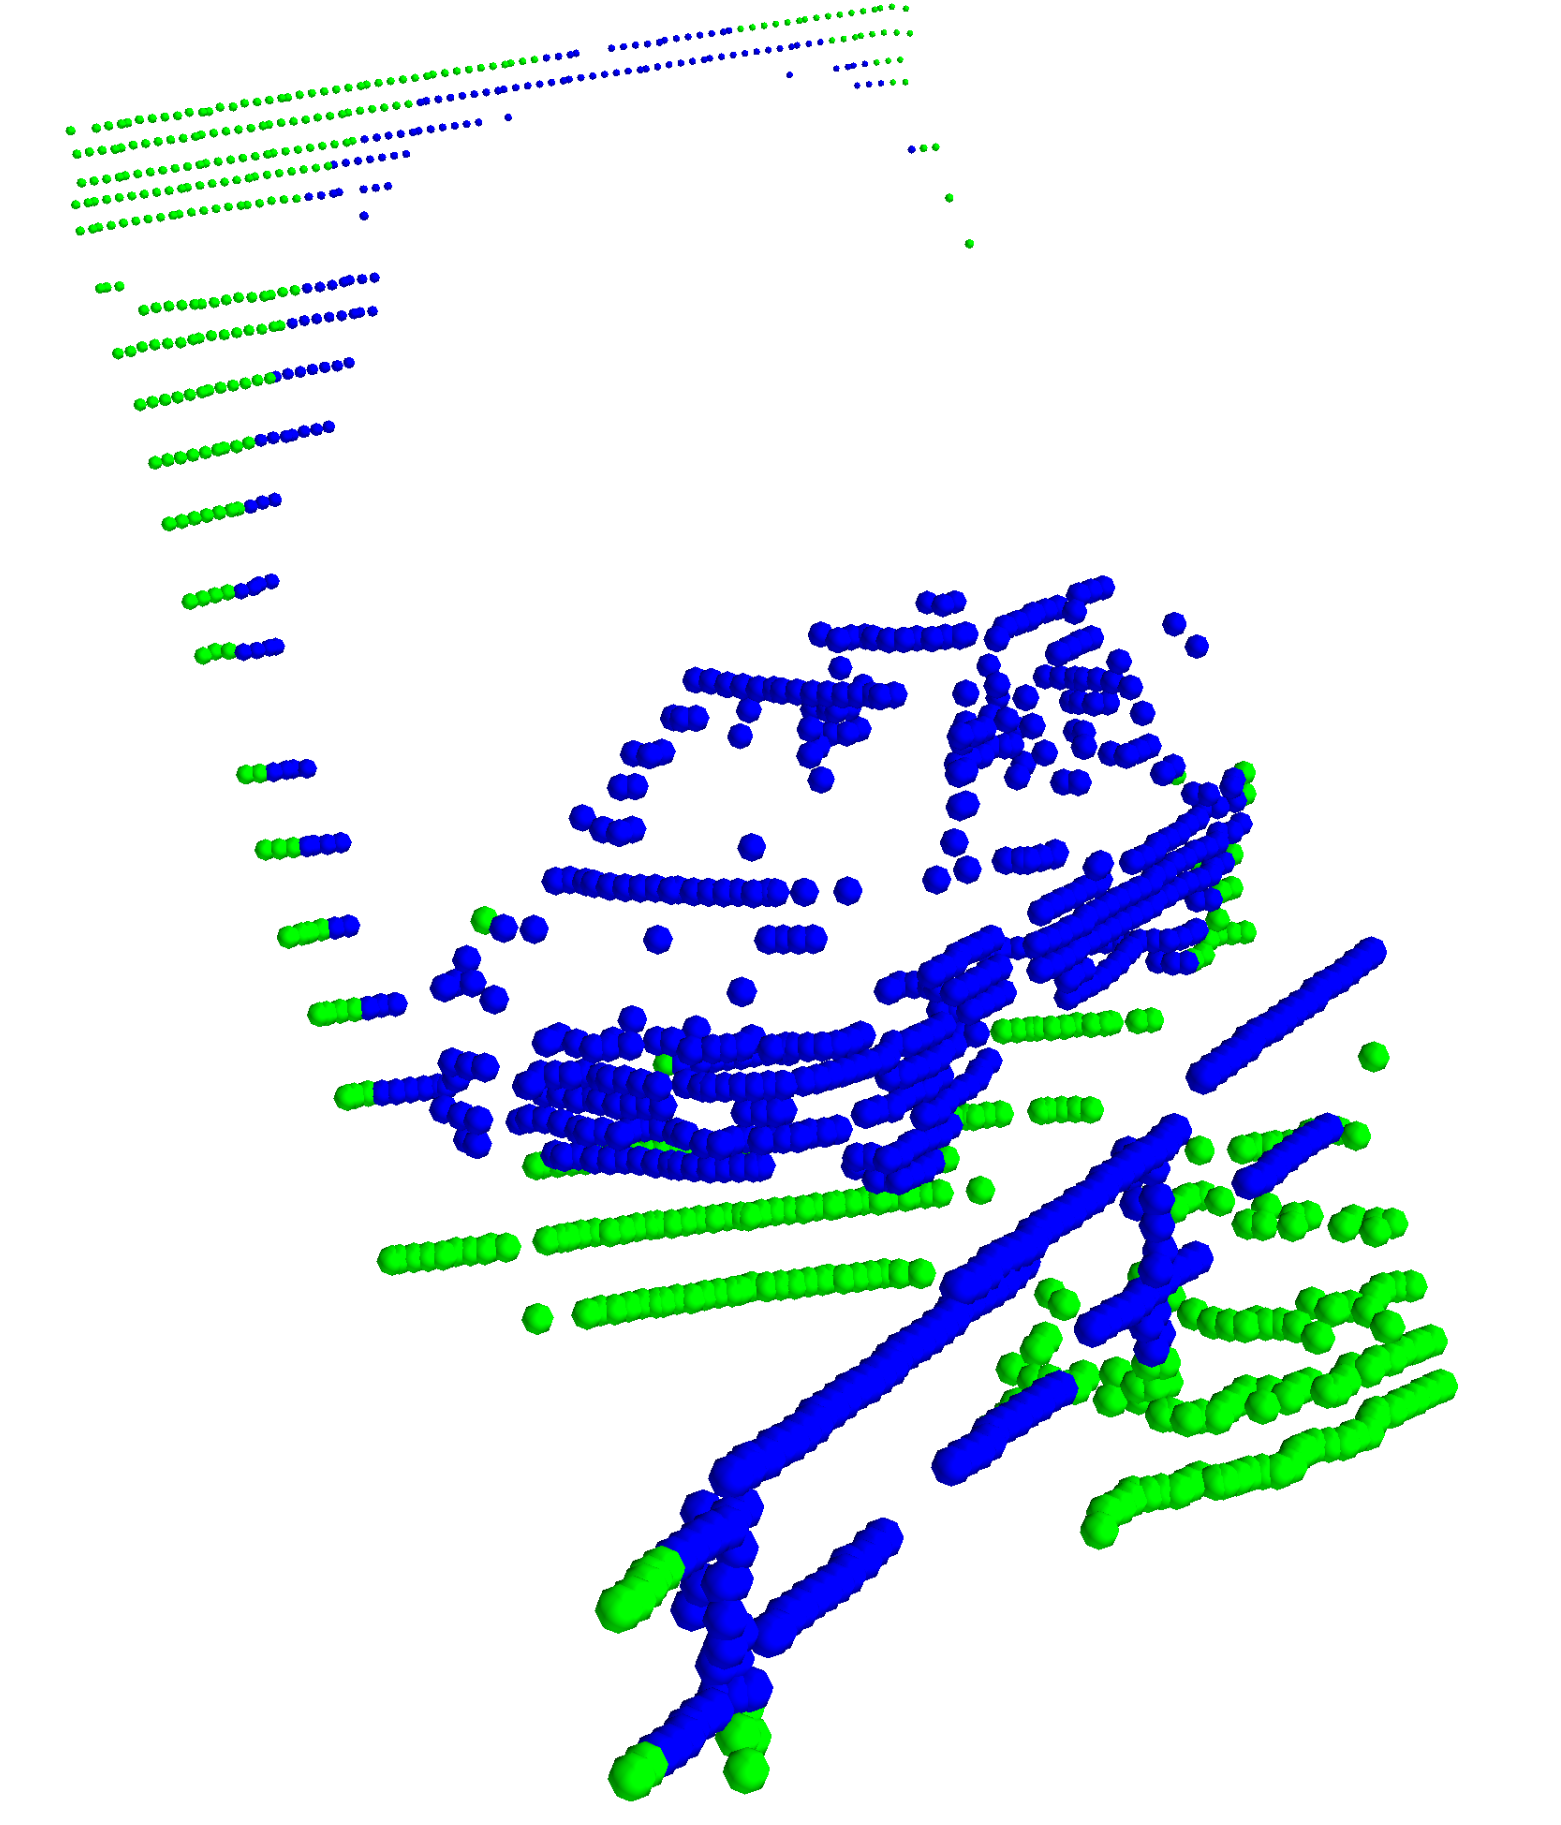
\includegraphics[width=0.2\textwidth]{figures/method/ambiguous/ex5/pcd.png}
        
    \end{tabular}
    
    \caption{Even with the pixel level Mask-RCNN detections our remaining pointclouds in blue can still have a lot of noise caused occluding objects or imperfect masks which cause problems for a chamfer distance like fit}
    \label{fig:dataset_example}
    
\end{figure}